% Options for packages loaded elsewhere
\PassOptionsToPackage{unicode}{hyperref}
\PassOptionsToPackage{hyphens}{url}
\PassOptionsToPackage{dvipsnames,svgnames,x11names}{xcolor}
%
\documentclass[
  letterpaper,
  DIV=11,
  numbers=noendperiod]{scrreprt}

\usepackage{amsmath,amssymb}
\usepackage{iftex}
\ifPDFTeX
  \usepackage[T1]{fontenc}
  \usepackage[utf8]{inputenc}
  \usepackage{textcomp} % provide euro and other symbols
\else % if luatex or xetex
  \usepackage{unicode-math}
  \defaultfontfeatures{Scale=MatchLowercase}
  \defaultfontfeatures[\rmfamily]{Ligatures=TeX,Scale=1}
\fi
\usepackage{lmodern}
\ifPDFTeX\else  
    % xetex/luatex font selection
\fi
% Use upquote if available, for straight quotes in verbatim environments
\IfFileExists{upquote.sty}{\usepackage{upquote}}{}
\IfFileExists{microtype.sty}{% use microtype if available
  \usepackage[]{microtype}
  \UseMicrotypeSet[protrusion]{basicmath} % disable protrusion for tt fonts
}{}
\makeatletter
\@ifundefined{KOMAClassName}{% if non-KOMA class
  \IfFileExists{parskip.sty}{%
    \usepackage{parskip}
  }{% else
    \setlength{\parindent}{0pt}
    \setlength{\parskip}{6pt plus 2pt minus 1pt}}
}{% if KOMA class
  \KOMAoptions{parskip=half}}
\makeatother
\usepackage{xcolor}
\setlength{\emergencystretch}{3em} % prevent overfull lines
\setcounter{secnumdepth}{5}
% Make \paragraph and \subparagraph free-standing
\ifx\paragraph\undefined\else
  \let\oldparagraph\paragraph
  \renewcommand{\paragraph}[1]{\oldparagraph{#1}\mbox{}}
\fi
\ifx\subparagraph\undefined\else
  \let\oldsubparagraph\subparagraph
  \renewcommand{\subparagraph}[1]{\oldsubparagraph{#1}\mbox{}}
\fi

\usepackage{color}
\usepackage{fancyvrb}
\newcommand{\VerbBar}{|}
\newcommand{\VERB}{\Verb[commandchars=\\\{\}]}
\DefineVerbatimEnvironment{Highlighting}{Verbatim}{commandchars=\\\{\}}
% Add ',fontsize=\small' for more characters per line
\usepackage{framed}
\definecolor{shadecolor}{RGB}{241,243,245}
\newenvironment{Shaded}{\begin{snugshade}}{\end{snugshade}}
\newcommand{\AlertTok}[1]{\textcolor[rgb]{0.68,0.00,0.00}{#1}}
\newcommand{\AnnotationTok}[1]{\textcolor[rgb]{0.37,0.37,0.37}{#1}}
\newcommand{\AttributeTok}[1]{\textcolor[rgb]{0.40,0.45,0.13}{#1}}
\newcommand{\BaseNTok}[1]{\textcolor[rgb]{0.68,0.00,0.00}{#1}}
\newcommand{\BuiltInTok}[1]{\textcolor[rgb]{0.00,0.23,0.31}{#1}}
\newcommand{\CharTok}[1]{\textcolor[rgb]{0.13,0.47,0.30}{#1}}
\newcommand{\CommentTok}[1]{\textcolor[rgb]{0.37,0.37,0.37}{#1}}
\newcommand{\CommentVarTok}[1]{\textcolor[rgb]{0.37,0.37,0.37}{\textit{#1}}}
\newcommand{\ConstantTok}[1]{\textcolor[rgb]{0.56,0.35,0.01}{#1}}
\newcommand{\ControlFlowTok}[1]{\textcolor[rgb]{0.00,0.23,0.31}{#1}}
\newcommand{\DataTypeTok}[1]{\textcolor[rgb]{0.68,0.00,0.00}{#1}}
\newcommand{\DecValTok}[1]{\textcolor[rgb]{0.68,0.00,0.00}{#1}}
\newcommand{\DocumentationTok}[1]{\textcolor[rgb]{0.37,0.37,0.37}{\textit{#1}}}
\newcommand{\ErrorTok}[1]{\textcolor[rgb]{0.68,0.00,0.00}{#1}}
\newcommand{\ExtensionTok}[1]{\textcolor[rgb]{0.00,0.23,0.31}{#1}}
\newcommand{\FloatTok}[1]{\textcolor[rgb]{0.68,0.00,0.00}{#1}}
\newcommand{\FunctionTok}[1]{\textcolor[rgb]{0.28,0.35,0.67}{#1}}
\newcommand{\ImportTok}[1]{\textcolor[rgb]{0.00,0.46,0.62}{#1}}
\newcommand{\InformationTok}[1]{\textcolor[rgb]{0.37,0.37,0.37}{#1}}
\newcommand{\KeywordTok}[1]{\textcolor[rgb]{0.00,0.23,0.31}{#1}}
\newcommand{\NormalTok}[1]{\textcolor[rgb]{0.00,0.23,0.31}{#1}}
\newcommand{\OperatorTok}[1]{\textcolor[rgb]{0.37,0.37,0.37}{#1}}
\newcommand{\OtherTok}[1]{\textcolor[rgb]{0.00,0.23,0.31}{#1}}
\newcommand{\PreprocessorTok}[1]{\textcolor[rgb]{0.68,0.00,0.00}{#1}}
\newcommand{\RegionMarkerTok}[1]{\textcolor[rgb]{0.00,0.23,0.31}{#1}}
\newcommand{\SpecialCharTok}[1]{\textcolor[rgb]{0.37,0.37,0.37}{#1}}
\newcommand{\SpecialStringTok}[1]{\textcolor[rgb]{0.13,0.47,0.30}{#1}}
\newcommand{\StringTok}[1]{\textcolor[rgb]{0.13,0.47,0.30}{#1}}
\newcommand{\VariableTok}[1]{\textcolor[rgb]{0.07,0.07,0.07}{#1}}
\newcommand{\VerbatimStringTok}[1]{\textcolor[rgb]{0.13,0.47,0.30}{#1}}
\newcommand{\WarningTok}[1]{\textcolor[rgb]{0.37,0.37,0.37}{\textit{#1}}}

\providecommand{\tightlist}{%
  \setlength{\itemsep}{0pt}\setlength{\parskip}{0pt}}\usepackage{longtable,booktabs,array}
\usepackage{calc} % for calculating minipage widths
% Correct order of tables after \paragraph or \subparagraph
\usepackage{etoolbox}
\makeatletter
\patchcmd\longtable{\par}{\if@noskipsec\mbox{}\fi\par}{}{}
\makeatother
% Allow footnotes in longtable head/foot
\IfFileExists{footnotehyper.sty}{\usepackage{footnotehyper}}{\usepackage{footnote}}
\makesavenoteenv{longtable}
\usepackage{graphicx}
\makeatletter
\def\maxwidth{\ifdim\Gin@nat@width>\linewidth\linewidth\else\Gin@nat@width\fi}
\def\maxheight{\ifdim\Gin@nat@height>\textheight\textheight\else\Gin@nat@height\fi}
\makeatother
% Scale images if necessary, so that they will not overflow the page
% margins by default, and it is still possible to overwrite the defaults
% using explicit options in \includegraphics[width, height, ...]{}
\setkeys{Gin}{width=\maxwidth,height=\maxheight,keepaspectratio}
% Set default figure placement to htbp
\makeatletter
\def\fps@figure{htbp}
\makeatother
\newlength{\cslhangindent}
\setlength{\cslhangindent}{1.5em}
\newlength{\csllabelwidth}
\setlength{\csllabelwidth}{3em}
\newlength{\cslentryspacingunit} % times entry-spacing
\setlength{\cslentryspacingunit}{\parskip}
\newenvironment{CSLReferences}[2] % #1 hanging-ident, #2 entry spacing
 {% don't indent paragraphs
  \setlength{\parindent}{0pt}
  % turn on hanging indent if param 1 is 1
  \ifodd #1
  \let\oldpar\par
  \def\par{\hangindent=\cslhangindent\oldpar}
  \fi
  % set entry spacing
  \setlength{\parskip}{#2\cslentryspacingunit}
 }%
 {}
\usepackage{calc}
\newcommand{\CSLBlock}[1]{#1\hfill\break}
\newcommand{\CSLLeftMargin}[1]{\parbox[t]{\csllabelwidth}{#1}}
\newcommand{\CSLRightInline}[1]{\parbox[t]{\linewidth - \csllabelwidth}{#1}\break}
\newcommand{\CSLIndent}[1]{\hspace{\cslhangindent}#1}

\KOMAoption{captions}{tableheading}
\makeatletter
\makeatother
\makeatletter
\@ifpackageloaded{bookmark}{}{\usepackage{bookmark}}
\makeatother
\makeatletter
\@ifpackageloaded{caption}{}{\usepackage{caption}}
\AtBeginDocument{%
\ifdefined\contentsname
  \renewcommand*\contentsname{Table of contents}
\else
  \newcommand\contentsname{Table of contents}
\fi
\ifdefined\listfigurename
  \renewcommand*\listfigurename{List of Figures}
\else
  \newcommand\listfigurename{List of Figures}
\fi
\ifdefined\listtablename
  \renewcommand*\listtablename{List of Tables}
\else
  \newcommand\listtablename{List of Tables}
\fi
\ifdefined\figurename
  \renewcommand*\figurename{Figure}
\else
  \newcommand\figurename{Figure}
\fi
\ifdefined\tablename
  \renewcommand*\tablename{Table}
\else
  \newcommand\tablename{Table}
\fi
}
\@ifpackageloaded{float}{}{\usepackage{float}}
\floatstyle{ruled}
\@ifundefined{c@chapter}{\newfloat{codelisting}{h}{lop}}{\newfloat{codelisting}{h}{lop}[chapter]}
\floatname{codelisting}{Listing}
\newcommand*\listoflistings{\listof{codelisting}{List of Listings}}
\makeatother
\makeatletter
\@ifpackageloaded{caption}{}{\usepackage{caption}}
\@ifpackageloaded{subcaption}{}{\usepackage{subcaption}}
\makeatother
\makeatletter
\@ifpackageloaded{tcolorbox}{}{\usepackage[skins,breakable]{tcolorbox}}
\makeatother
\makeatletter
\@ifundefined{shadecolor}{\definecolor{shadecolor}{rgb}{.97, .97, .97}}
\makeatother
\makeatletter
\makeatother
\makeatletter
\makeatother
\makeatletter
\@ifpackageloaded{tikz}{}{\usepackage{tikz}}
\makeatother
        \newcommand*\circled[1]{\tikz[baseline=(char.base)]{
          \node[shape=circle,draw,inner sep=1pt] (char) {{\scriptsize#1}};}}  
                  
\ifLuaTeX
  \usepackage{selnolig}  % disable illegal ligatures
\fi
\IfFileExists{bookmark.sty}{\usepackage{bookmark}}{\usepackage{hyperref}}
\IfFileExists{xurl.sty}{\usepackage{xurl}}{} % add URL line breaks if available
\urlstyle{same} % disable monospaced font for URLs
\hypersetup{
  pdftitle={AE-WGAN-GP},
  pdfauthor={Davide Messina},
  colorlinks=true,
  linkcolor={blue},
  filecolor={Maroon},
  citecolor={Blue},
  urlcolor={Blue},
  pdfcreator={LaTeX via pandoc}}

\title{AE-WGAN-GP}
\author{Davide Messina}
\date{2024-03-10}

\begin{document}
\maketitle
\ifdefined\Shaded\renewenvironment{Shaded}{\begin{tcolorbox}[borderline west={3pt}{0pt}{shadecolor}, sharp corners, enhanced, boxrule=0pt, interior hidden, frame hidden, breakable]}{\end{tcolorbox}}\fi

\renewcommand*\contentsname{Table of contents}
{
\hypersetup{linkcolor=}
\setcounter{tocdepth}{2}
\tableofcontents
}
\bookmarksetup{startatroot}

\hypertarget{introduction}{%
\chapter{Introduction}\label{introduction}}

Some people say that we are currently living in the Information Age.

In many fields there is nowadays a necessity to have representative
synthetic data for multiple reasons:

\begin{enumerate}
\def\labelenumi{\arabic{enumi})}
\item
  By simulating actual data characteristics and patterns, they are able
  to mimic real-world scenarios correctly. Such sets empower researchers
  to query the dataset and expect an accurate response by impersonating
  features and trends of true data
\item
  They help researchers overcome limitations and ethical concerns that
  are usually associated with using real data. At times, privacy,
  security or legal restrictions could limit access to authentic data.
  By utilizing synthetic data these concerns can be alleviated.
\end{enumerate}

The path I took to develop the AE-WGAN-GP model from scratch has been
quite a journey.

I will attempt to replicate the informal style and tone found in some
medium post.

In the first chapter I will explain the general idea I had in the
beginning and the preprocessing of the data.

The second chapter talks about the AutoEncoder

In the third chapter I describe how I setup Colab and Git

Finally in the last chapter contains everything regarding the GAN

\bookmarksetup{startatroot}

\hypertarget{references}{%
\chapter*{References}\label{references}}
\addcontentsline{toc}{chapter}{References}

\markboth{References}{References}

\hypertarget{refs}{}
\begin{CSLReferences}{1}{0}
\leavevmode\vadjust pre{\hypertarget{ref-MedGAN}{}}%
Choi, Edward, Siddharth Biswal, Bradley Malin, Jon Duke, Walter F.
Stewart, and Jimeng Sun. 2018. {``Generating Multi-Label Discrete
Patient Records Using Generative Adversarial Networks,''} no.
arXiv:1703.06490 (January).
\url{https://doi.org/10.48550/arXiv.1703.06490}.

\leavevmode\vadjust pre{\hypertarget{ref-gulrajani2017improved}{}}%
Gulrajani, Ishaan, Faruk Ahmed, Martin Arjovsky, Vincent Dumoulin, and
Aaron Courville. 2017. {``Improved Training of Wasserstein GANs.''}
\url{https://arxiv.org/abs/1704.00028}.

\leavevmode\vadjust pre{\hypertarget{ref-ConcePTION}{}}%
Thurin et, al. 2022. {``From Inception to ConcePTION: Genesis of a
Network to Support Better Monitoring and Communication of Medication
Safety During Pregnancy and Breastfeeding.''} \emph{Clinical
Pharmacology \& Therapeutics} 111 (1): 321--31.
\url{https://doi.org/10.1002/cpt.2476}.

\end{CSLReferences}

\part{Introduction}

\hypertarget{medgan}{%
\chapter{MedGAN}\label{medgan}}

The original MedGAN article (Choi et al. 2018) was written by Choi et
al.~in 2017 and descrived for the first time a way to generate realistic
synthetic patient records.

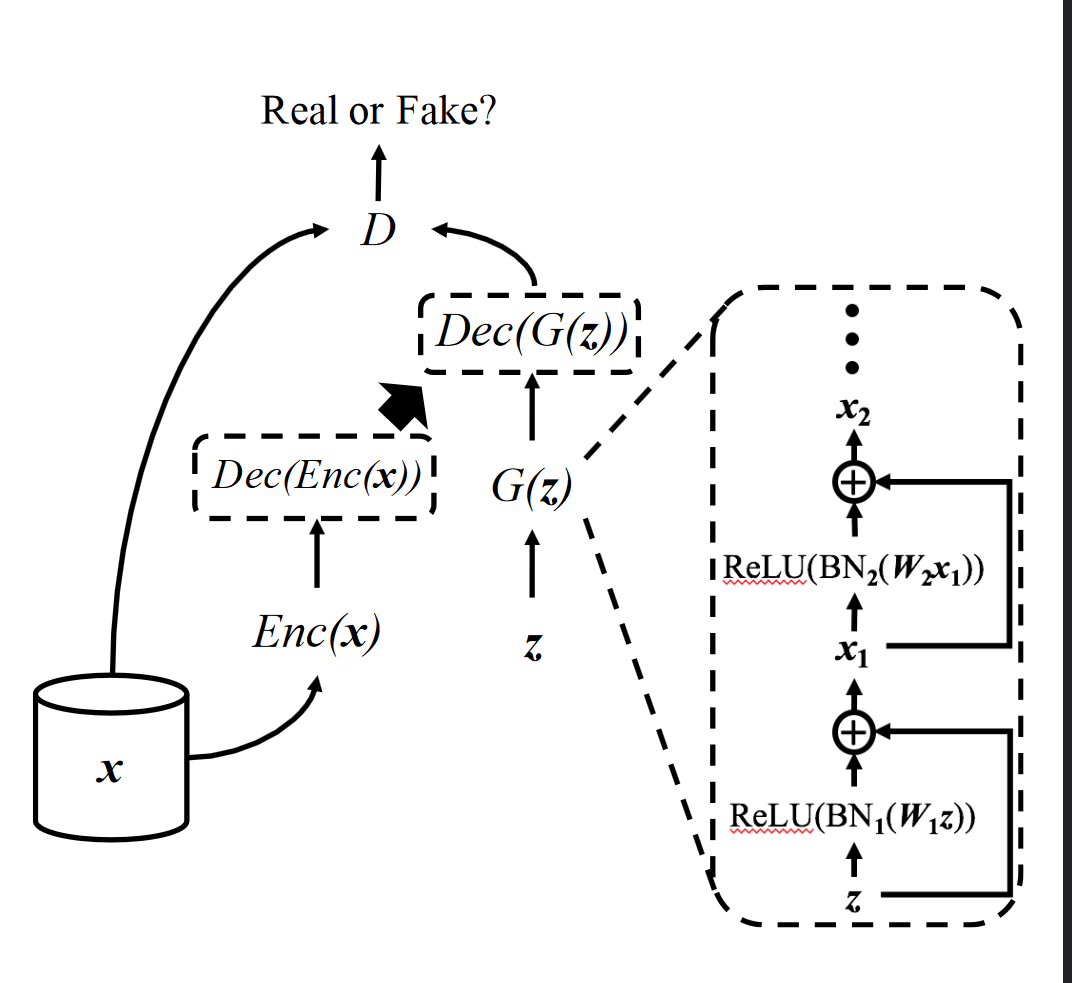
\includegraphics{MedGan.png} The idea was simple train: an autoencoder
on the original data and then use its decoder as part of the generator
of a GAN network to gnerate synthetic data.

My initial idea was to modify the input of the network proposed in the
original paper to ingest my dataset, maybe play a little with activation
functions and optimizers to find the optimal implementation for my use
case.

\begin{figure}

{\centering 
\includegraphics{medgan-meme.jpg}

}

\caption{Boy, was I wrong!}

\end{figure}

\hypertarget{cdm-and-data-instance}{%
\chapter{CDM and Data instance}\label{cdm-and-data-instance}}

ConcePTION(see Thurin et 2022) is an IMI project which began in 2019. As
one of the project outputs, ConcePTION aimed to establish a trusted
ecosystem that generates and disseminates reliable, evidence-based
information regarding effects of medication used during pregnancy and
breastfeeding. To this end, a CDM was designed to manage, within
constrained timelines and budget, the heterogeneity inherent in the
diverse data sources in Europe.

The ConcePTION CDM includes 16 tables. Each table includes multiple
variables. The picture below summarises the ConcePTION CDM.

As you can see, the tables have four different colours. The colours
indicate the four types of data tables:

\begin{itemize}
\tightlist
\item
  Green: Routine healthcare data, such as data related to medical events
  (diagnoses/symptoms), medicines, vaccines, medical procedures and
  medical observations.
\item
  Dark blue: Surveillance data, such as registries (birth registries,
  congenital anomaly registries, disease registries, \ldots), surveys or
  cohorts.
\item
  Light blue: Curated data, such as demographics, observation periods
  and person relationships (e.g., mother/child linkage).
\item
  Grey: Metadata, i.e., information regarding the data in the model,
  such as extraction dates and drugs detailed definition.
\end{itemize}

Linkages between the different tables are represented by lines:

\begin{itemize}
\tightlist
\item
  Solid black lines: The linkages across records of the same person
  (e.g., patient demographics from Persons table to diagnosis codes from
  Events table).
\item
  Dotted lines: The linkages across items extracted from the same record
  (e.g., hospital stays from Visit occurrence table to diagnosis codes
  from Events table).
\item
  Solid grey lines: The linkages from items referring to a medicinal
  product or vaccines to the full product description in the Product
  table.
\end{itemize}

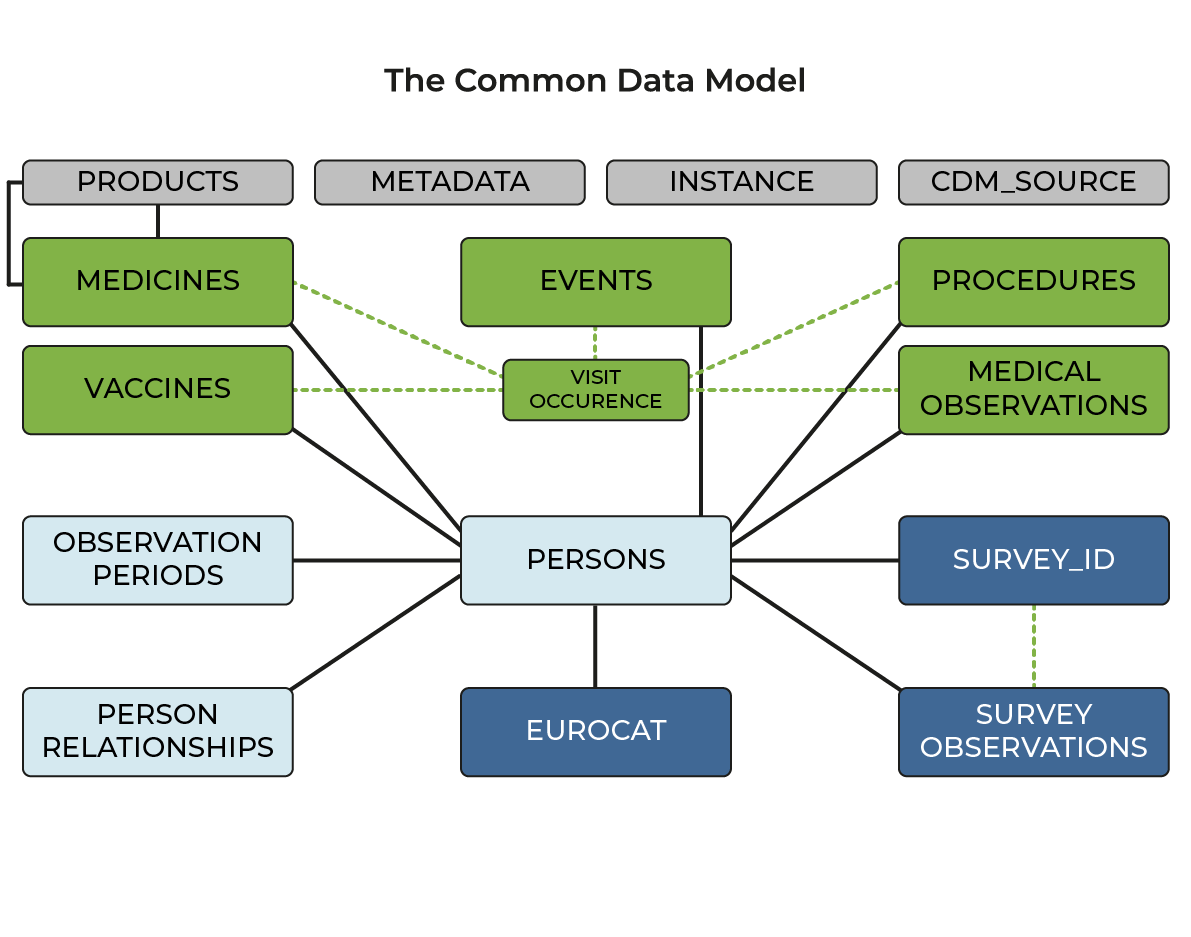
\includegraphics{Common Data Model.png}

A data instance of a CDM refers to a set of structured data that
conforms to the predefined schema and semantics.

To train the AE-WGAN-GP I used synthetic data since for privacy concerns
I could used real data.

The instance I used is available
\href{https://github.com/dado330/AE-WGAN-GP/tree/main/R_preprocessing/i_input_subpop}{here}.

\hypertarget{preprocessing-using-r}{%
\chapter{Preprocessing using R}\label{preprocessing-using-r}}

In the previous section I explained how a data instance of the
ConcePTION CDM is a complex object.

Defining a model which would generate an entire instance is outside the
scope of this project and even SOTA models have not arrived there yet.

Using an R script I firstly extracted all conceptsets defined in the
codelist available
\href{https://github.com/dado330/AE-WGAN-GP/blob/main/R_preprocessing/p_parameters/archive_parameters/20231127_V2_full_codelist_at_20231127.csv}{here}

I then created variables based on those conceptsets and finally a
dataset which contains records of persons positive to 18 certain events
in the year prior to a specific moment. A person obviously might have
more than one event in that period of time.

Some of the more rare events are being excluded since the dataset size
is small and training the model would be too complicated if those would
have been retained.

These are the final dataset characteristic:

\begin{itemize}
\tightlist
\item
  719 rows
\item
  18 columns representing the 18 final events:

  \begin{itemize}
  \tightlist
  \item
    B\_COAGDIS\_AESI
  \item
    C\_ARRH\_AESI
  \item
    C\_CAD\_AESI
  \item
    C\_MYOCARD\_AESI
  \item
    C\_VALVULAR\_AESI
  \item
    DEATH
  \item
    D\_PANCRACUTE\_AESI
  \item
    E\_DM1\_AESI
  \item
    E\_GOUT\_AESI
  \item
    G\_KIACUTE\_AESI
  \item
    G\_UTI\_AESI
  \item
    I\_INFLUENZA\_AESI
  \item
    M\_FRACTURES\_AESI
  \item
    M\_OSTEOARTHRITIS\_AESI
  \item
    N\_STROKEHEMO\_AESI
  \item
    SO\_OTITISEXT\_AESI
  \item
    V\_THROMBOSISARTERIALALGOR\_AESI
  \item
    V\_VTEALGORITHM\_AESI
  \end{itemize}
\item
  All 18 columns are binary variable with 1 =\textgreater{} the person
  had the event, 0 =\textgreater{} otherwise
\item
  28 records with 3 events, 52 records with 2 events and the remaining
  with 1 event
\item
  Some rare event, f.e. N\_STROKEHEMO\_AESI with 10 records
\item
  A very common event which is DEATH with 258 records
\end{itemize}

To finish the preprocessing I transformed the dataset to Numpy array
ready to be ingested in Python

\hypertarget{local-environment-setup}{%
\chapter{Local environment setup}\label{local-environment-setup}}

First thing I needed to do after having generated the input data for the
network was to install python.

I went to \href{https://www.python.org/downloads/}{Python website},
downloaded the latest release and then installed it. After installation
I updated the
\href{https://datatofish.com/add-python-to-windows-path/}{Windows PATH}
and upgrade pip from CMD.

I then installed PyCharm as IDE through a student license and proceed to
install all necessary packages. Especially
\href{https://www.tensorflow.org/}{TensorFlow}.

Here, I got my first error:

Could not find a version that satisfies the requirement TensorFlow (from
versions: ) No matching distribution found for TensorFlow.

After digging in Stack Overflow I found what the problem really was:
TensorFlow was not yet available for the latest python version. I then
downgraded python and reinstalled all packages, TensorFlow included this
time.

After running a sample TensorFlow script in noticed two messages that
appears every time I would import the module

I tensorflow/core/util/port.cc:113{]} oneDNN custom operations are on.
You may see slightly different numerical results due to floating-point
round-off errors from different computation orders. To turn them off,
set the environment variable \texttt{TF\_ENABLE\_ONEDNN\_OPTS=0}.

I tensorflow/core/platform/cpu\_feature\_guard.cc:210{]} This TensorFlow
binary is optimized to use available CPU instructions in
performance-critical operations. To enable the following instructions:
SSE SSE2 SSE3 SSE4.1 SSE4.2, in other operations, rebuild TensorFlow
with the appropriate compiler flags.

After a little bit of research I found the first one was not very
important.

The second one is a suggestion to use optimized instruction sets even
not in performance-critical operations. I left this one as is because I
first wanted to have a feel on the training time and as a last resort
compile TensorFlow to take advantage of those instruction sets. In
addition my CPU is a fairly old I3-3220 without even AVX2 support so I
thought the difference would be negligible anyway.

\part{AE}

\hypertarget{why-an-autoencoder-in-a-gan}{%
\chapter{Why an AutoEncoder in a
GAN?}\label{why-an-autoencoder-in-a-gan}}

In general the main advantage of AutoEncoders (AE) is the dimensionality
reduction of its input. This compact representation then force the
network to learn the salient features of the initial data.

However using an autoencoder in combination with a GAN has several
additional benefits which in my opinion are more important:

\begin{enumerate}
\def\labelenumi{\arabic{enumi}.}
\item
  Help Generator Training: The generator in a GAN learns to generate
  realistic samples by fooling the discriminator. The autoencoder acts
  as a pre-training mechanism for the generator since it won't need to
  learn to generate discrete data but only salient features for the
  decoder.
\item
  Regularization: Incorporating an autoencoder as part of a GAN
  architecture can act as a regularization technique since it acts as an
  additional constraint for the generator by forcing it to generate
  samples that can be accurately reconstructed. This helps in avoiding
  mode collapse.
\end{enumerate}

More on this topics later on in the GAN chapter.

\hypertarget{original-code-is-unusable}{%
\chapter{Original code is unusable}\label{original-code-is-unusable}}

After installing Python and TensorFlow I was ready to run some code.

The MedGAN paper provides the souce code in a GitHub repository
\href{https://github.com/mp2893/medgan}{here} and my first idea was to
reuse that.

I cloned the repo on my local machine and I started changing it to be
able to ingest my initial data. I removed the CMD listener found in the
script and transform my R data into a Numpy matrix.

Finally I tried running the script but I soon found a sad reality: the
script was built using TensorFlow V1.\\
I tried disabling eager execution but to no avail: I was then made aware
that to run this script I would have needed to update possibly many of
its functions to their newer V2 versions which might be retroactively
compatible.

\begin{figure}

{\centering 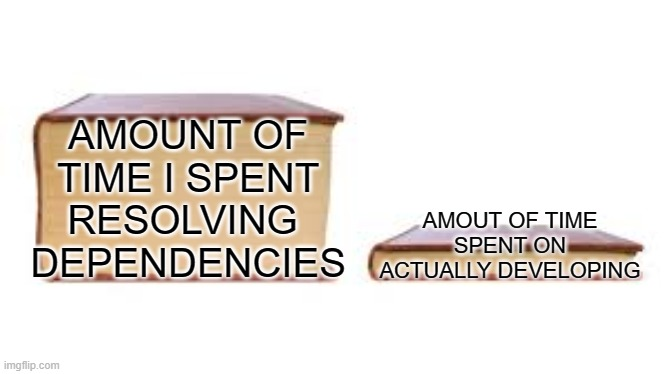
\includegraphics{upgrade_TF.png}

}

\caption{This is what I feared would have happened}

\end{figure}

I then decided to find another, more recent, implementation of the
MedGAN network, possibly implemented by a third party.\\
I searched trough forks with updated code but to no avail.

I then made an extensive search on GitHub and found this repository:
\href{https://github.com/yy6linda/synthetic-ehr-benchmarking}{Benchmarking
framework of synthetic electronic health record generation models}.\\
Inside the repo there is a
\href{https://github.com/yy6linda/synthetic-ehr-benchmarking/blob/main/data_generation/vumc/medgan_vumc.py}{file}
containing the MedGAN network and I decided it would have been easier to
update that script since it was much more recent than the previous one.

\hypertarget{fixing-what-found-in-github}{%
\chapter{Fixing what found in
GitHub}\label{fixing-what-found-in-github}}

After cloning the new repo I tried analyzing the script to understand
what it was doing and the reason behind each actions.

I made a few observation and changes:

\begin{itemize}
\tightlist
\item
  The input data in this case was not a Numpy matrix but a series of
  Numpy arrays.\\
  I then changed accordingly the procedure to transform the R data in
  the Numpy object.
\item
  The original paper works with count or binary variables (XOR) while
  this script utilizes both at the same times./ I'm going to discuss
  this topic in the AE and WGAN-GP sections.
\item
  The class AdamWeightDecay defined in the script was not working
  correctly so I just switched to AdamW function defined in
  tf.keras.optimizers since it didn't seem to me the original class was
  doing anything special.
\item
  The argument \textbf{\emph{interpolation}} of the function
  Numpy.nanpercentile() has been deprecated so I changed to
  \textbf{\emph{method}} after looking at the documentation online.
\item
  The script was creating 5 different models. I only needed one so I
  removed a cycle.
\item
  Changed paths of both the input data and output files
\end{itemize}

After this I was ready to train the MedGAN on my data (or so I
thought\ldots)

\hypertarget{running-the-autoencoder-for-the-first-time}{%
\chapter{Running the AutoEncoder for the first
time}\label{running-the-autoencoder-for-the-first-time}}

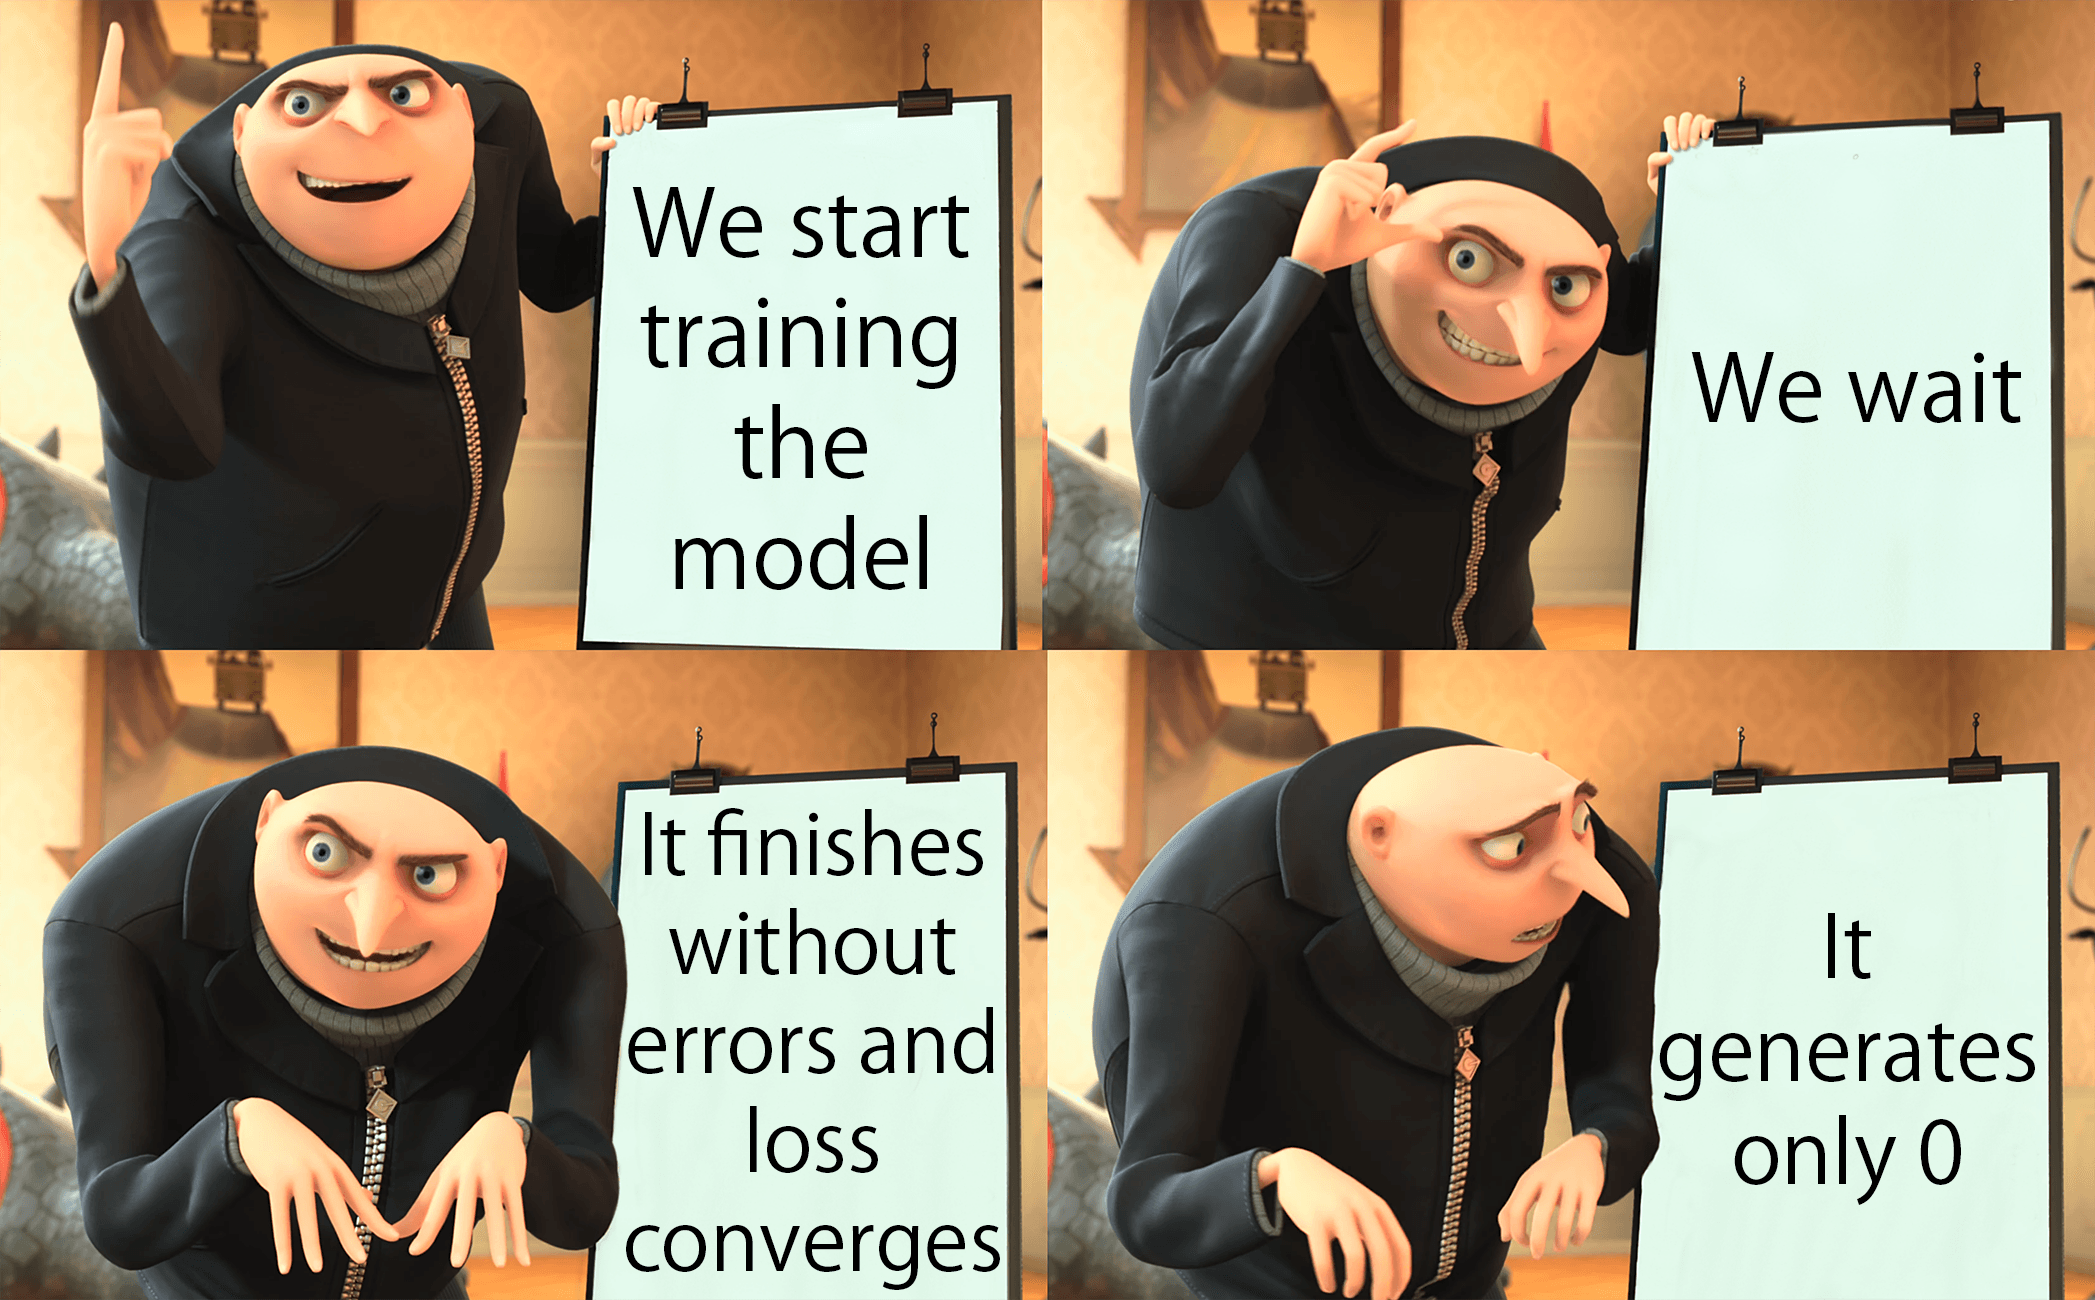
\includegraphics{ae_0.png}

Above is pretty much my reaction when I trained for the first time the
AE. The loss did converges but it wasn't near zero at all so the model
was not learning properly.

To help visualizing what was going on I added a piece of code that would
print the current batch, synthetic and then real data.

\hypertarget{annotated-cell-9}{%
\label{annotated-cell-9}}%
\begin{Shaded}
\begin{Highlighting}[]
\ControlFlowTok{if}\NormalTok{ np.random.uniform(size}\OperatorTok{=}\DecValTok{1}\NormalTok{) }\OperatorTok{\textgreater{}} \FloatTok{0.99}\NormalTok{:  }\hspace*{\fill}\NormalTok{\circled{1}}
  \BuiltInTok{print}\NormalTok{(}\StringTok{"synthetic"}\NormalTok{)                  }\hspace*{\fill}\NormalTok{\circled{2}}
  \BuiltInTok{print}\NormalTok{(tf.}\BuiltInTok{round}\NormalTok{(synthetic).numpy())  }
  \BuiltInTok{print}\NormalTok{(}\StringTok{"real"}\NormalTok{)                       }\hspace*{\fill}\NormalTok{\circled{3}}
  \BuiltInTok{print}\NormalTok{(real.numpy())                 }
\end{Highlighting}
\end{Shaded}

\begin{description}
\tightlist
\item[\circled{1}]
Every 1 out 100 batches do
\item[\circled{2}]
Print the reconstructed data
\item[\circled{3}]
Print the original data
\end{description}

I then noticed how the generated data initially had more frequent events
as 1 for all of the records then after some time they suddenly become 0
one after the other. This was clearly not ideal.

\hypertarget{activations-of-output-layer-of-encoder}{%
\chapter{Activations of output layer of
Encoder}\label{activations-of-output-layer-of-encoder}}

I started reviewing the Encoder and the Decoder to find macroscopic
mistakes or something wrong at a glance. I didn't noticed anything in
particular so I started reading the MedGAN paper to look for clues.

I subsequently noticed how the activation function of the output layer I
used for the Encoder was a sigmoid while in the paper was a hyperbolic
tangent (Tanh).\\
I changed it and the loss decreased from 800\textasciitilde1000 to
around 500\textasciitilde700. All the values were still 0, they were
just converging to 0 faster probably.

It's almost always preferable to use Tanh instead of sigmoid as action
function whenever it is possible. An example of when it is better to use
the sigmoid is in our case as activation function of the Decoder's
output layer: each value of our original data (so our ideal output) is 0
or 1, since the sigmoid output values from 0 to 1 this is a perfect fit.
On the other hand it is not important what is the output of the Encoder.
The Encoder map the original input onto a latent space which it is not
necessary to be restricted to the range {[}0, 1{]}

The reason the Tanh is in general better than the sigmoid is simple: the
outputs of the Tanh are zero-centered.\\
This translates in easier and more stable training for the model.

Obviously the model as of right now it's still useless so I still
continued to fine tune the network.

\hypertarget{hyperparameters}{%
\chapter{Hyperparameters}\label{hyperparameters}}

I then started improving the model by carefully testing combinations of
hyperparameters because:


\includegraphics{pick_hyperparameters.png}

I've tried multiple times to changes parameters some of them are:

\begin{itemize}
\tightlist
\item
  Number of models trained:\\
  Maybe the model is not stable and every instance may result in very
  different final losses.
\item
  Increase layers size and networks depth:\\
  The Encoder and Decoder may not have the capabilities to learn
  correctly because there aren't sufficient nodes/connections between
  them.
\item
  Decreasing learning rate γ, β1 or β2:\\
  If the model is learning too quickly it might be overshooting and the
  loss may be bouncing around its minimum without really decreasing.
\item
  Increasing learning rate γ, β1 or β2:\\
  If the model is learning too slowly it can get stuck in a local
  minima.
\item
  Change batch size:\\
  Less important than previous points. In theory larger batches should
  decrease learning rate but make the model more consistent, the other
  way around for smaller batches. No real changes in my opinion in this
  case. I didn't really think this would have been a solution since the
  model was already consistent but converging to a not good enough
  state.
\item
  Batch normalization:\\
  Centering and scaling the input of a layer should make the model
  converge faster and more stable.
\item
  Activation function of inner layers (and Batch normalization):\\
  I tried using Selu as activation function instead of Relu to add
  internal normalization and to not remove negative weights.
\end{itemize}

In the sections I will explain what worked in my case.

\hypertarget{expanding-the-models}{%
\chapter{Expanding the models}\label{expanding-the-models}}

At this point I was quite desperate to have something at least usable so
I decide to increase the size of the Encoder and Decoder.

I left both the networks with 3 hidden layers ans started increasing the
size of each layer.

At the beginning the Encoder had layers with 18, 32, 64, 128, 256 units
while the Decoder 256, 128, 64, 32, 18.\\
I then begin to double the size of each layer in hope this would help
the model train (except the 18 which is fixed)

As a summary:

\begin{itemize}
\tightlist
\item
  Maximum size 256, loss: 500\textasciitilde700
\item
  Maximum size 512, loss: 500
\item
  Maximum size 1024, loss: 500
\item
  Maximum size 2048, loss: 500
\item
  Maximum size 4096, loss: 500
\end{itemize}

The loss remain pretty much the same, just more consistent and faster in
reaching the lower bound found in more parsimonious models. Everything
is still 0.

\hypertarget{custom-loss}{%
\chapter{Custom loss}\label{custom-loss}}

Following the paper I originally used the binary cross-entropy as loss
function of the AutoEncoder. At this point, however, I had the idea to
modify it to better suit my data.

After some thought my hypothesis was:

\begin{enumerate}
\def\labelenumi{\arabic{enumi}.}
\tightlist
\item
  The dataset is sparse. There are only a few ``1'' values with respect
  to ``0'' values.
\item
  This problem might be exacerbated by the sparse nature of the more
  uncommon events.
\item
  The loss which is the Binary Cross Entropy in theory should handle
  class imbalance but maybe not on sparse data.
\end{enumerate}

I tried then to think about a possible solution:

\begin{enumerate}
\def\labelenumi{\arabic{enumi}.}
\tightlist
\item
  The loss is generated by values which are 0 but should be 1, never the
  other way around
\item
  Maybe the loss is not penalizing enough the case when 0 should be a 1
\item
  Which function can penalizes values near 0 but not near 1? The Log is
  a good candidate
\item
  I first tried to take the negative Log of the syntetic data and
  obviously everything degenerated to 1
\item
  I then thought to compare the synthetic and real data: if they are
  both the same then the loss should be 0
\end{enumerate}

My final solution was:

\[
- Ln(mean(synthetic + e^{-10})) + Ln(mean(real))
\]

This formula penalizes when the sum of the synthetic data is lower than
the one on real data. The loss is especially larger when the sum of the
synthetic data is near 0.

There are more refined approaches to this problem but this seemed to
work.\\
(Note: I needed to add the exponential to make the model more robust.
Otherwise in case the syntethic data in the batch was all 0 at any point
it would be impossible for the loss to be calculated)

Using this formula as a loss penalty in addition to the binary
cross-entropy I was able to get the loss of the model with maximum size
4096 to around 200. Now the model partially encode and decode correctly
some of the variables. Those variables are in general the more common
events, the rarer events remain at 0.

This is still not sufficient and I tried different approaches in next
sections

\hypertarget{activations-of-hidden-layers-of-ae}{%
\chapter{Activations of hidden layers of
AE}\label{activations-of-hidden-layers-of-ae}}

Both the Encoder and the Decoder used Relu as activation function of
their hidden layers. Relu is easy to calculate but at the same time
negative inputs turns to 0 instantaneously.

Using Tanh as activation function of the output layer of the Encoder
means it is possible to have negative values as output so we might want
to change the Relus to something else.

I choosed to try leaky Relu but there were no major changes between this
and Relu. I then decided to use Tanh as activation layer of the hidden
layers too.\\
This change was very impactful and the loss became 0 very fast.

Using 4096 as maximum size of the model previously increased the
computation time to around 40s so this may not be feasible when will
train the GAN so I decided to train and decrease the size of the models.

As a summary:

\begin{itemize}
\tightlist
\item
  Maximum size 4096, loss: \textasciitilde0
\item
  Maximum size 2048, loss: \textasciitilde0
\item
  Maximum size 1024, loss: \textasciitilde8 (but on test data
  \textasciitilde20)
\item
  Maximum size 512, loss: \textasciitilde25 (but on test data
  \textasciitilde50)
\item
  Maximum size 256, loss: \textasciitilde250
\end{itemize}

To get those loss values I needed to gradually increase then number of
epochs, from 50 for the 4096 size to 1000 for the 256 size.

In an effort to increase performance I then implemented Batch
Normalization (BN) after each hidden layer but without notable results.

Since changing the activation function of the hidden layer has such a
big impact I decided to make a new attempt.\\
I tried to use more unusual activations and found Selu to be very good.
This maybe be caused by the self-normalizing nature of the activation
function which works better than BN in this case.

With Selu I could get Encoder and Decoder with maximum size 512 to have
0 loss and train much faster in less than 50 epochs compared to 400 with
Tanh

Using 256 as maximum size still left me with around 40\textasciitilde80
loss.

I thought of the possibility to change the activation function of the
Encoder's output layer too to Selu but I was unsure if that would
creating problems in the GAN. The Selu didn't seem symmetric so taking a
sample from a Normal distribution might not be ideal (Increasing the
difficulty in training the Generator)

\hypertarget{miscellaneous-hyperparameters}{%
\chapter{Miscellaneous
Hyperparameters}\label{miscellaneous-hyperparameters}}

As optimizers I left what was already there, so AdamW.

I used different learning rates during the previous training but in
general:

\begin{itemize}
\tightlist
\item
  0.0001 the first 3 epochs
\item
  0.00006 between 4 and 10 epochs
\item
  0.00003 between 11 and 20 epochs
\item
  0.00001 after 21 epochs
\end{itemize}

The higher learning rate at the beginning is used to speed up the
training while the lower learning rate at the end is to fine tune the
model.

I slightly decreased β\textsubscript{1} to help lowering the learning
rate.

I decreased weight decay too, to be consistent with the lower learning
rate.

\hypertarget{bad-model-vs-bad-model}{%
\chapter{Bad model vs Bad model}\label{bad-model-vs-bad-model}}

The model until now it's working very well but it is because it clearly
overfitting.

I then tried to create models with lower or same units as the input but
they couldn't recreate the original data well.

It was necessary to decide if I should use the overfitting model (Model
A) or the not accurate one (Model B)

\begin{figure}

{\centering 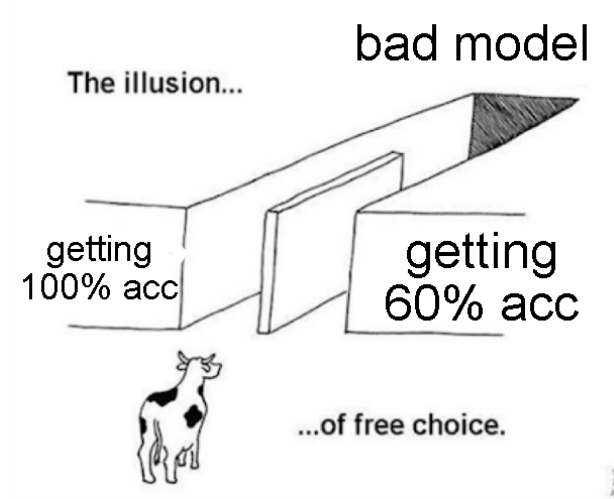
\includegraphics{overfitting.png}

}

\caption{The problem I was facing could be summarized by this image}

\end{figure}

In general it is better to use neither of them, obviously, but in our
case which is the worse model?

The issue with the model A is that it is probably only capable of
reconstructing data very similar to the training data.

The models B on the other hand don't encode and decode the more uncommon
event at all. They are treated as not existent.

The objective of the MedGAN (and AE-WGAN-GP) is to generate synthetic
data similar to the original one. With model A the data will be very
similar almost identical to the original while model B won't create
uncommon variables as they will always be 0.

This crucial in our case since in epidemiological studies we are often
more interested in rare events since there is less information regarding
them in the litereature.

Taking into account the above mentioned reasons I decided to use model
A, so the overfitting one.

\part{COLAB}

\hypertarget{why-use-google}{%
\chapter{Why use Google}\label{why-use-google}}

This chapter explain my switch from PyCharm to Google Colab.

In reality this happen just after running the GAN on my PC. Before with
the AE the maximum running time was around 40 minutes however the GAN
surpassed the psychological threshold of 1 hour so I decided to find a
faster solution.


\includegraphics{skeleton.jpg}

Searching a solution to optimize my code made me stumble on Google
Colab. Google Colab is a free cloud-based Jupyter notebook environment
that runs on Google infrastructure. It allows users to run Python
scripts in a browser-based interface, with access to GPUs (with
caveats).

\begin{figure}

{\centering 
\includegraphics{hulk gpu.png}

}

\caption{How I felt after discovering Google Colab}

\end{figure}

That was perfect for me! In addition to have the possibility to run my
models on a GPU I could already generate my plots and results on a
Jupyter notebook which I could then share and Google Colab provides
pre-installed libraries for ML and data analysis so no more problems
with Python and libraries versions mess.

I then started setting up the environment and understanding how to make
my script works on Colab

\hypertarget{setup-on-drive}{%
\chapter{Setup on Drive}\label{setup-on-drive}}

The first thing I did was copying what I already have done inside cells
on Colab. I then uploaded my input dataset on the VM and modified the
path inside the script.

After a day has passed with me cleaning the script and rerunning the
AutoEncoder on Colab I found out the VM state is not saved once you are
disconnected from it.

The easiest solution and the one sponsored By Google is to use Google
Drive.

Next, I uploaded the input data on my Google Drive which is then mounted
the VM on Colab using the following command (and by giving many
permissions)

\begin{Shaded}
\begin{Highlighting}[]
\ImportTok{from}\NormalTok{ google.colab }\ImportTok{import}\NormalTok{ drive}
\NormalTok{drive.mount(‘}\OperatorTok{/}\NormalTok{content}\OperatorTok{/}\NormalTok{gdrive’)}
\end{Highlighting}
\end{Shaded}

I changed again the path to the input files (and checkpoints) and rerun
again the AutoEncoder.

\hypertarget{setup-git}{%
\chapter{Setup Git}\label{setup-git}}

At some point I wanted to test the script on my local machine before
running it in Colab (see next chapter and section) but copying the files
was redundant and prone to errors.\\
In addition I discovered that once I shared my notebook with some else
directly from Colab all outputs will be lost.

The solution to these problems I arrived was using Git, a distributed
version control system.

Firstly, I opened a GitHub repository and from my local machine I
uploaded the preprocessing and the input data.\\
On the VM the process is slightly more difficult:

\begin{enumerate}
\def\labelenumi{\arabic{enumi}.}
\tightlist
\item
  I setup my credentials and path to GitHub. Credentials are to used
  only during the push to GitHub
\end{enumerate}

\begin{Shaded}
\begin{Highlighting}[]
\NormalTok{GIT\_USERNAME }\OperatorTok{=} \StringTok{"dado330"}
\NormalTok{GIT\_MAIL }\OperatorTok{=} \StringTok{"messina.davide.statistician@gmail.com"}
\NormalTok{GIT\_REPO }\OperatorTok{=} \StringTok{"https://github.com/dado330/AE{-}WGAN{-}GP"}
\end{Highlighting}
\end{Shaded}

\begin{enumerate}
\def\labelenumi{\arabic{enumi}.}
\setcounter{enumi}{1}
\tightlist
\item
  I cloned the repository on the VM. I didn't need any form of
  authentication since the repo is public.
\end{enumerate}

\begin{Shaded}
\begin{Highlighting}[]
\OperatorTok{!}\NormalTok{git clone $GIT\_REPO}
\end{Highlighting}
\end{Shaded}

\begin{enumerate}
\def\labelenumi{\arabic{enumi}.}
\setcounter{enumi}{2}
\tightlist
\item
  I inserted a cell to pull changes I've tested locally.
\end{enumerate}

\begin{Shaded}
\begin{Highlighting}[]
\OperatorTok{\%\%}\NormalTok{bash}
\NormalTok{cd }\OperatorTok{/}\NormalTok{content}\OperatorTok{/}\NormalTok{AE}\OperatorTok{{-}}\NormalTok{WGAN}\OperatorTok{{-}}\NormalTok{GP}
\NormalTok{git pull origin main}
\end{Highlighting}
\end{Shaded}

\begin{enumerate}
\def\labelenumi{\arabic{enumi}.}
\setcounter{enumi}{3}
\tightlist
\item
  This cell makes Git aware of our credentials
\end{enumerate}

\begin{Shaded}
\begin{Highlighting}[]
\OperatorTok{!}\NormalTok{git config }\OperatorTok{{-}{-}}\KeywordTok{global}\NormalTok{ user.email $GIT\_MAIL}
\OperatorTok{!}\NormalTok{git config }\OperatorTok{{-}{-}}\KeywordTok{global}\NormalTok{ user.name $GIT\_USERNAME}
\end{Highlighting}
\end{Shaded}

\begin{enumerate}
\def\labelenumi{\arabic{enumi}.}
\setcounter{enumi}{4}
\tightlist
\item
  To push changes we need a token. You can easily generate one in your
  GitHub account with at least Repo scope. (For example:
  ghp\_rlAAU4Kz1toabuGbkTauF9sYCg4pRf1CMm0q).\\
  Then set the origin where to push the commits to a combinations of
  token and repository link as below.
\end{enumerate}

\begin{Shaded}
\begin{Highlighting}[]
\OperatorTok{\%\%}\NormalTok{bash}
\NormalTok{cd }\OperatorTok{/}\NormalTok{content}\OperatorTok{/}\NormalTok{AE}\OperatorTok{{-}}\NormalTok{WGAN}\OperatorTok{{-}}\NormalTok{GP}
\NormalTok{git remote }\BuiltInTok{set}\OperatorTok{{-}}\NormalTok{url origin }\StringTok{"https://ghp\_rlAAU4Kz1toabuGbkTauF9sYCg4pRf1CMm0q@github.com/dado330/AE{-}WGAN{-}GP.git"}
\end{Highlighting}
\end{Shaded}

\begin{enumerate}
\def\labelenumi{\arabic{enumi}.}
\setcounter{enumi}{5}
\tightlist
\item
  Here I stage all changes. Commit them with a message and then push the
  commit to the origin defined previously.
\end{enumerate}

\begin{Shaded}
\begin{Highlighting}[]
\OperatorTok{\%\%}\NormalTok{bash}
\NormalTok{cd }\OperatorTok{/}\NormalTok{content}\OperatorTok{/}\NormalTok{AE}\OperatorTok{{-}}\NormalTok{WGAN}\OperatorTok{{-}}\NormalTok{GP}
\NormalTok{git add }\OperatorTok{{-}}\NormalTok{A}
\NormalTok{git commit }\OperatorTok{{-}}\NormalTok{m }\StringTok{"Updated comments and generated data"}
\NormalTok{git push }\OperatorTok{{-}}\NormalTok{u origin main}
\end{Highlighting}
\end{Shaded}

The Jupyter notebook was saved on the repository using the internal
options of Google Colab.

Now all files related to the projects are publicly accessible and
included the notebook's outputs.

\hypertarget{drawbacks-and-final-summary}{%
\chapter{Drawbacks and final
summary}\label{drawbacks-and-final-summary}}

One of the reason to make a first run on my local machine before running
the model on Colab was the time limit imposed the virtual machine
instance by Google.

After 12 hours the disconnection is automatic but it often happens
before that limit if Google feel that you are not interacting with the
session anymore.

\begin{figure}

{\centering \includegraphics{colab_sleep.webp}

}

\caption{This is how I felt}

\end{figure}

If I needed to be away from my PC I used a software to emulate key
strokes, mouse movements and clicks.

The real issue when I was working and in the meantime the model was
running on Colab in the background, a situation which happened most of
the times.\\
In this situation it happened multiple times that my session
disconnected while the model was still training.

Another reason to use Colab was to have access to a GPU to train my
models.\\
I discovered after testing that GANs do not really take advantage of the
computational power of a GPU so I was quite bummed out. It was not
uncommon to have a GPU instance slower than a CPU one.\\
There was also a huge variance between VM instances with respect to
running time of the models: it could happen that opening a new VM would
double the computation time of each epochs with changing any
parameters.\\
In addition since the VM's resources we are with are shared between
multiple user on a single server there is a penalty in performance. The
time it takes to run the model on Colab is comparable to what my PC is
capable of using an I3 from more than 10 years ago and DDR3.

To summarize my experience with google Colab I would say:

Positive:

\begin{itemize}
\tightlist
\item
  Python environment already setup. No need check python or package
  dependencies/versions, GPU drivers, etc..
\item
  Use Jupyter notebook
\item
  Do not use local machine resources which can then be used for other
  tasks
\item
  Machine has a discrete amount of RAM to run the model (more than the
  16GB on my PC)
\end{itemize}

Neutral:

\begin{itemize}
\tightlist
\item
  Sharing the notebook from within Colab will lose all output but there
  is a solution by using Git
\item
  There is a penalty in the performance with respect to the same machine
  running the same model locally
\end{itemize}

Negative:

\begin{itemize}
\tightlist
\item
  Variance in performance between VM instances of the same class
\item
  Disconnections are possible even before the 12 hours limit
\item
  Once your session is disconnected all data not saved somewhere else
  are lost
\end{itemize}

\part{GAN}

\hypertarget{running-the-gan-for-the-first-time}{%
\chapter{Running the GAN for the first
time}\label{running-the-gan-for-the-first-time}}

Now it is time to run the GAN and try to really simulate our synthetic
data.

In the previous chapter ``Fixing what found in GitHub'' I already
discussed what I changed before the first run.\\
In addition I needed the changed the output of the Generator to be 512
units, in line with what is the input of the Decoder.

I started running the model and these were my observation:

\begin{enumerate}
\def\labelenumi{\arabic{enumi}.}
\tightlist
\item
  At the very beginning there a moderate decrease in Generator while the
  Discriminator stayed pretty much the same
\item
  The Generator loss continued to decrease and the Discriminator one
  started to increase
\item
  This trend was not linear in both networks
\item
  After some time the Discriminator loss started to decrease and the
  Generator one to increase
\item
  The Discriminator loss converged to a very small number while the
  Generator loss converged to a value higher than the starting point
\item
  I then tried to generate some synthetic data using the trained
  Generator but I discovered how it only generated observation with the
  event DEATH which is the most common one
\item
  The GAN was mode collapsing (see point 6)
\end{enumerate}

The next section will explain mode collapsing.

\hypertarget{mode-collapse}{%
\chapter{Mode Collapse}\label{mode-collapse}}


\includegraphics{morty_collapse.jpg}

Mode collapsing happens when the generator produce only a subset of the
patters or modes found in the original distribution.\\
In our case all outputs are persons which have as event DEATH.

To understand why the model is mode collapsing I should describe in
general how a GAN works

The idea is to use Generator to create a vector on the latent space
generated by the Encoder and use the Decoder to convert those values
which will then be compared, by the discriminator, to an original
sample.

The issue is, many times, the Discriminator is much more powerful than
the Generator: the Generator won't have time to learn all the features
before the Discriminator became too good and prevents the Generator to
further improve its performance.

Obviously I didn't want the GAN to mode collapse so I tried find
solutions

\hypertarget{tentative-solutions}{%
\chapter{Tentative solutions}\label{tentative-solutions}}

At the beginning I analyzed what I found in the repository and compared
it to the original MedGAN paper. I quickly noticed how the Generator was
incomplete since the shortcut connections were missing.

In addition I tried:

\begin{itemize}
\tightlist
\item
  Increasing Generator number of layers (size of the layer is fixed by
  Decoder and shortcut connections)
\item
  Increasing Discriminator number and size of layers. (best results by
  first increasing size and then decreasing it slowly)
\item
  Decreasing learning rate and β and weight decay in Discriminator (and
  Generator indipendently)
\item
  Define a penalty to the Binary Cross Entropy in both Generator and
  Discriminator losses
\item
  Retrain the AutoEncoder to increase the size of the Generator
\item
  Regularization with L1
\item
  Switch activation function from Relu to Selu
\item
  Train the Generator N times each epoch while only once for the
  Discriminator. In the original paper was the other way around.
\end{itemize}

With some combination of hyperparameters I had the impression it was
training better and more stable but I couldn't get it to stop mode
collapsing in the end.

\hypertarget{training-wgan-gp}{%
\chapter{Training WGAN-GP}\label{training-wgan-gp}}

After running the WGAN-GP on a limited number of epochs I could quickly
tell that it was working.\\
This was probably possible by the changes previously done to the
networks when I was testing GAN and WGAN.

I then decided to halve the learning rate of both Generator and
Discriminator and increase the number of epochs to 20000 to obtain the
best possible result.

Finally I was able to train the final model in around 6 hours on Colab.
The final model was then saved on the repository as checkpoint using
git.

This final model's discriminator loss reached a state of bouncing around
0, so small enough, and consequently the trained Generator should be
quite good, as explained before.\\
The generator loss was around -3700 but that does not influence the
model performance at all so it is not a metric for it.

\hypertarget{wgan}{%
\chapter{WGAN}\label{wgan}}

I tried searching for an easier model to train and I found the WGAN.\\
It promises improve stability and less probability of diverging.

This is possible because this time we are not constraining the generator
but only the discriminator. At the same time what we want to use from
the WGAN in the end is the Generator to create synthetic data.

But if we are not defining a loss function how can we evaluate the
Generator performance?

\begin{figure}

{\centering 
\includegraphics{no_loss.PNG}

}

\caption{It's easy!}

\end{figure}

Another very important advantage of WGAN over traditional GAN is that
the discriminator loss function should be connected to the quality of
the simulated data using that model and consequently easier to
interpret. Lower loss values should translate in better generation of
synthetic data.

However, I quickly discovered how even with the vanilla WGAN I had
problems in getting useful results because, in addition to the
hyperparameters defined in the previous section, I needed to setup the
clipping factor of the weights that enforces the Lipschitz constraint.

I had the impression fine tuning that parameter wouldn't be easy. At the
same time the WGAN was a clear improvement over the simple GAN so I
tried to find other researches/articles in how to setup correctly the
clipping factor.

\hypertarget{wgan-gp}{%
\chapter{WGAN-GP}\label{wgan-gp}}

Searching for WGAN models tutorials lead me to the a derivative model
called WGAN-GP from an example in the
\href{https://keras.io/examples/generative/wgan_gp/}{Keras
documentation}.

The original was easy to find here: (Gulrajani et al. 2017)

Here the enforcing of the Lipschitz constraints is not done by clipping
weights but in alternative way through a gradient penalty. This a softer
version of the original constraint since we want the weights to converge
to 1 and not simply clip them as before.

In the code from Keras documentation the generate the interpolated data
for the gradient penalty by calculating the difference between generated
and real data multiplied by a variable sampled from a uniform(0, 1)
which is then added to the real data.\\
In the original paper however the first term is added to the generated
image. I'm not sure why this is setup as such in the example but I
changed it to reflect what is inside the manuscript.

In addition in the WGAN-GP they highlight how to not use batch
normalization in the Discriminator so I removed all of them. In their
stead I decide to use the Selu which normalize internally.\\

For the gradient penalty coefficient λ I decided to retain what is
specified in the paper, so 10. Same treatment for learning rates, βs and
number of times the Discriminator is trained each epoch.

\hypertarget{results}{%
\chapter{Results}\label{results}}

Using the Generator I created a dataset 1000 times larger than the
initial one.

\begin{figure}

{\centering 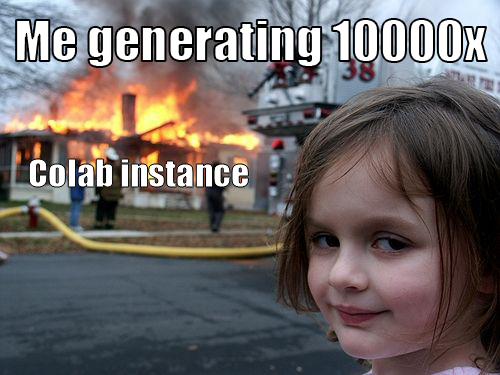
\includegraphics{10000x.png}

}

\caption{10000 Times didn't work\ldots{}}

\end{figure}

The Generator is not perfect so some of its output contains only 0.
Since that is clearly impossible I decided to remove those rows. In
total they were less than 2\% of the generated dataset.

I then calculated the mean number of cases for each events I would get
if I generated a dataset of the same size as the initial one

\begin{longtable}[]{@{}
  >{\raggedright\arraybackslash}p{(\columnwidth - 8\tabcolsep) * \real{0.4638}}
  >{\raggedright\arraybackslash}p{(\columnwidth - 8\tabcolsep) * \real{0.1159}}
  >{\raggedright\arraybackslash}p{(\columnwidth - 8\tabcolsep) * \real{0.1884}}
  >{\raggedright\arraybackslash}p{(\columnwidth - 8\tabcolsep) * \real{0.1594}}
  >{\raggedright\arraybackslash}p{(\columnwidth - 8\tabcolsep) * \real{0.0725}}@{}}
\toprule\noalign{}
\begin{minipage}[b]{\linewidth}\raggedright
Varnames
\end{minipage} & \begin{minipage}[b]{\linewidth}\raggedright
0\_real
\end{minipage} & \begin{minipage}[b]{\linewidth}\raggedright
0\_synthetic
\end{minipage} & \begin{minipage}[b]{\linewidth}\raggedright
diff\_perc
\end{minipage} & \begin{minipage}[b]{\linewidth}\raggedright
\end{minipage} \\
\midrule\noalign{}
\endhead
\bottomrule\noalign{}
\endlastfoot
B\_COAGDIS\_AESI & 73.0 & 73.715309 & -0.98 & \\
C\_ARRH\_AESI & 65.0 & 69.045921 & -6.22 & \\
C\_CAD\_AESI & 31.0 & 31.479591 & -1.55 & \\
C\_MYOCARD\_AESI & 20.0 & 17.986734 & 10.07 & \\
C\_VALVULAR\_AESI & 50.0 & 51.130611 & -2.26 & \\
DEATH & 258.0 & 253.684692 & 1.67 & \\
D\_PANCRACUTE\_AESI & 13.0 & 9.452041 & 27.29 & \\
E\_DM1\_AESI & 38.0 & 44.208164 & -16.34 & \\
E\_GOUT\_AESI & 27.0 & 25.344898 & 6.13 & \\
G\_KIACUTE\_AESI & 15.0 & 14.710204 & 1.93 & \\
G\_UTI\_AESI & 23.0 & 23.219387 & -0.95 & \\
I\_INFLUENZA\_AESI & 16.0 & 14.138776 & 11.63 & \\
M\_FRACTURES\_AESI & 60.0 & 59.522449 & 0.80 & \\
M\_OSTEOARTHRITIS\_AESI & 28.0 & 27.116327 & 3.16 & \\
N\_STROKEHEMO\_AESI & 10.0 & 9.992857 & 0.07 & \\
SO\_OTITISEXT\_AESI & 36.0 & 37.114285 & -3.10 & \\
V\_THROMBOSISARTERIALALGOR\_AESI & 45.0 & 45.730614 & -1.62 & \\
V\_VTEALGORITHM\_AESI & 19.0 & 19.263266 & -1.39 & \\
\end{longtable}

The script reproduce well most of the variables. However
D\_PANCRACUTE\_AESI, C\_MYOCARD\_AESI and I\_INFLUENZA\_AESI are
slightly underrepresented in the generated data, while E\_DM1\_AESI on
the other hand is over represented.

The Mean Square Error is 5.63 which is good enough in this case.

Finally I wantef to see the number of events each persons has:

\begin{longtable}[]{@{}llll@{}}
\toprule\noalign{}
Number of events & 0\_real & 0\_synthetic & diff\_perc \\
\midrule\noalign{}
\endhead
\bottomrule\noalign{}
\endlastfoot
1.0 & 639 & 639.180612 & -0.03 \\
2.0 & 52 & 52.792857 & -1.52 \\
3.0 & 28 & 27.562245 & 1.56 \\
\end{longtable}

The script does a very good job in this case. I removed the impossible
cases when the person has 0 events but even with that taken into account
the performance does not drop much.

The Mean Square Error is only 0.28 which is very good.



\end{document}
